\chapter{The Trial}

At eight o’clock in the morning Albert had arrived at Beauchamp’s door.
The valet de chambre had received orders to usher him in at once.
Beauchamp was in his bath.

“Here I am,” Albert said.

“Well, my poor friend,” replied Beauchamp, “I expected you.”

“I need not say I think you are too faithful and too kind to have
spoken of that painful circumstance. Your having sent for me is another
proof of your affection. So, without losing time, tell me, have you the
slightest idea whence this terrible blow proceeds?”

“I think I have some clew.”

“But first tell me all the particulars of this shameful plot.”

Beauchamp proceeded to relate to the young man, who was overwhelmed
with shame and grief, the following facts. Two days previously, the
article had appeared in another paper besides \textit{ l’Impartial}, and, what
was more serious, one that was well known as a government paper.
Beauchamp was breakfasting when he read the paragraph. He sent
immediately for a cabriolet, and hastened to the publisher’s office.
Although professing diametrically opposite principles from those of the
editor of the other paper, Beauchamp—as it sometimes, we may say often,
happens—was his intimate friend. The editor was reading, with apparent
delight, a leading article in the same paper on beet-sugar, probably a
composition of his own.

“Ah, \textit{pardieu!}” said Beauchamp, “with the paper in your hand, my
friend, I need not tell you the cause of my visit.”

“Are you interested in the sugar question?” asked the editor of the
ministerial paper.

“No,” replied Beauchamp, “I have not considered the question; a totally
different subject interests me.”

“What is it?”

“The article relative to Morcerf.”

“Indeed? Is it not a curious affair?”

“So curious, that I think you are running a great risk of a prosecution
for defamation of character.”

“Not at all; we have received with the information all the requisite
proofs, and we are quite sure M. de Morcerf will not raise his voice
against us; besides, it is rendering a service to one’s country to
denounce these wretched criminals who are unworthy of the honor
bestowed on them.”

Beauchamp was thunderstruck.

“Who, then, has so correctly informed you?” asked he; “for my paper,
which gave the first information on the subject, has been obliged to
stop for want of proof; and yet we are more interested than you in
exposing M. de Morcerf, as he is a peer of France, and we are of the
opposition.”

“Oh, that is very simple; we have not sought to scandalize. This news
was brought to us. A man arrived yesterday from Yanina, bringing a
formidable array of documents; and when we hesitated to publish the
accusatory article, he told us it should be inserted in some other
paper.”

Beauchamp understood that nothing remained but to submit, and left the
office to despatch a courier to Morcerf. But he had been unable to send
to Albert the following particulars, as the events had transpired after
the messenger’s departure; namely, that the same day a great agitation
was manifest in the House of Peers among the usually calm members of
that dignified assembly. Everyone had arrived almost before the usual
hour, and was conversing on the melancholy event which was to attract
the attention of the public towards one of their most illustrious
colleagues. Some were perusing the article, others making comments and
recalling circumstances which substantiated the charges still more.

The Count of Morcerf was no favorite with his colleagues. Like all
upstarts, he had had recourse to a great deal of haughtiness to
maintain his position. The true nobility laughed at him, the talented
repelled him, and the honorable instinctively despised him. He was, in
fact, in the unhappy position of the victim marked for sacrifice; the
finger of God once pointed at him, everyone was prepared to raise the
hue and cry.

The Count of Morcerf alone was ignorant of the news. He did not take in
the paper containing the defamatory article, and had passed the morning
in writing letters and in trying a horse. He arrived at his usual hour,
with a proud look and insolent demeanor; he alighted, passed through
the corridors, and entered the house without observing the hesitation
of the door-keepers or the coolness of his colleagues.

\begin{figure}[ht]
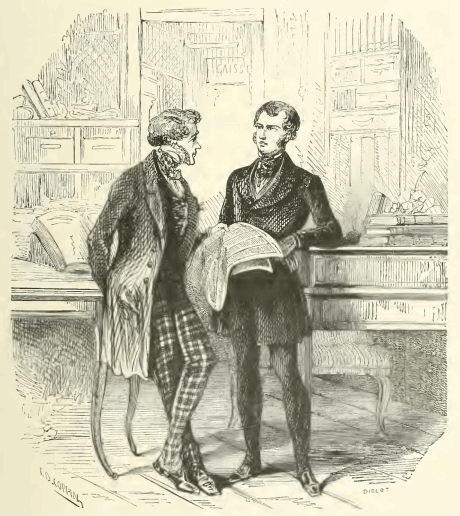
\includegraphics[width=\textwidth]{40194m.jpg}
\end{figure}

Business had already been going on for half an hour when he entered.
Everyone held the accusing paper, but, as usual, no one liked to take
upon himself the responsibility of the attack. At length an honorable
peer, Morcerf’s acknowledged enemy, ascended the tribune with that
solemnity which announced that the expected moment had arrived. There
was an impressive silence; Morcerf alone knew not why such profound
attention was given to an orator who was not always listened to with so
much complacency.

The count did not notice the introduction, in which the speaker
announced that his communication would be of that vital importance that
it demanded the undivided attention of the House; but at the mention of
Yanina and Colonel Fernand, he turned so frightfully pale that every
member shuddered and fixed his eyes upon him. Moral wounds have this
peculiarity,—they may be hidden, but they never close; always painful,
always ready to bleed when touched, they remain fresh and open in the
heart.

The article having been read during the painful hush that followed, a
universal shudder pervaded the assembly, and immediately the closest
attention was given to the orator as he resumed his remarks. He stated
his scruples and the difficulties of the case; it was the honor of M.
de Morcerf, and that of the whole House, he proposed to defend, by
provoking a debate on personal questions, which are always such painful
themes of discussion. He concluded by calling for an investigation,
which might dispose of the calumnious report before it had time to
spread, and restore M. de Morcerf to the position he had long held in
public opinion.

Morcerf was so completely overwhelmed by this great and unexpected
calamity that he could scarcely stammer a few words as he looked around
on the assembly. This timidity, which might proceed from the
astonishment of innocence as well as the shame of guilt, conciliated
some in his favor; for men who are truly generous are always ready to
compassionate when the misfortune of their enemy surpasses the limits
of their hatred.

The president put it to the vote, and it was decided that the
investigation should take place. The count was asked what time he
required to prepare his defence. Morcerf’s courage had revived when he
found himself alive after this horrible blow.

“My lords,” answered he, “it is not by time I could repel the attack
made on me by enemies unknown to me, and, doubtless, hidden in
obscurity; it is immediately, and by a thunderbolt, that I must repel
the flash of lightning which, for a moment, startled me. Oh, that I
could, instead of taking up this defence, shed my last drop of blood to
prove to my noble colleagues that I am their equal in worth.”

These words made a favorable impression on behalf of the accused.

“I demand, then, that the examination shall take place as soon as
possible, and I will furnish the house with all necessary information.”

“What day do you fix?” asked the president.

“Today I am at your service,” replied the count.

The president rang the bell. “Does the House approve that the
examination should take place today?”

\begin{figure}[ht]
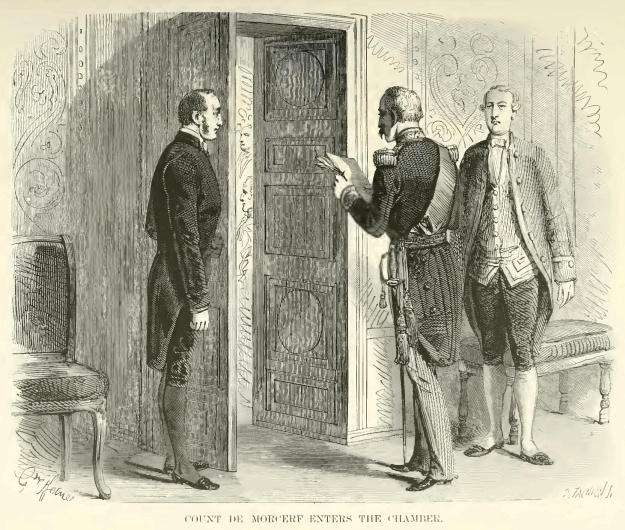
\includegraphics[width=\textwidth]{40196m.jpg}
\end{figure}

“Yes,” was the unanimous answer.

A committee of twelve members was chosen to examine the proofs brought
forward by Morcerf. The investigation would begin at eight o’clock that
evening in the committee-room, and if postponement were necessary, the
proceedings would be resumed each evening at the same hour. Morcerf
asked leave to retire; he had to collect the documents he had long been
preparing against this storm, which his sagacity had foreseen.

Beauchamp related to the young man all the facts we have just narrated;
his story, however, had over ours all the advantage of the animation of
living things over the coldness of dead things.

Albert listened, trembling now with hope, then with anger, and then
again with shame, for from Beauchamp’s confidence he knew his father
was guilty, and he asked himself how, since he was guilty, he could
prove his innocence. Beauchamp hesitated to continue his narrative.

“What next?” asked Albert.

“What next? My friend, you impose a painful task on me. Must you know
all?”

“Absolutely; and rather from your lips than another’s.”

“Muster up all your courage, then, for never have you required it
more.”

Albert passed his hand over his forehead, as if to try his strength, as
a man who is preparing to defend his life proves his shield and bends
his sword. He thought himself strong enough, for he mistook fever for
energy. “Go on,” said he.

“The evening arrived; all Paris was in expectation. Many said your
father had only to show himself to crush the charge against him; many
others said he would not appear; while some asserted that they had seen
him start for Brussels; and others went to the police-office to inquire
if he had taken out a passport. I used all my influence with one of the
committee, a young peer of my acquaintance, to get admission to one of
the galleries. He called for me at seven o’clock, and, before anyone
had arrived, asked one of the door-keepers to place me in a box. I was
concealed by a column, and might witness the whole of the terrible
scene which was about to take place. At eight o’clock all were in their
places, and M. de Morcerf entered at the last stroke. He held some
papers in his hand; his countenance was calm, and his step firm, and he
was dressed with great care in his military uniform, which was buttoned
completely up to the chin. His presence produced a good effect. The
committee was made up of Liberals, several of whom came forward to
shake hands with him.”

Albert felt his heart bursting at these particulars, but gratitude
mingled with his sorrow: he would gladly have embraced those who had
given his father this proof of esteem at a moment when his honor was so
powerfully attacked.

“At this moment one of the door-keepers brought in a letter for the
president. ‘You are at liberty to speak, M. de Morcerf,’ said the
president, as he unsealed the letter; and the count began his defence,
I assure you, Albert, in a most eloquent and skilful manner. He
produced documents proving that the Vizier of Yanina had up to the last
moment honored him with his entire confidence, since he had interested
him with a negotiation of life and death with the emperor. He produced
the ring, his mark of authority, with which Ali Pasha generally sealed
his letters, and which the latter had given him, that he might, on his
return at any hour of the day or night, gain access to the presence,
even in the harem. Unfortunately, the negotiation failed, and when he
returned to defend his benefactor, he was dead. ‘But,’ said the count,
‘so great was Ali Pasha’s confidence, that on his death-bed he resigned
his favorite mistress and her daughter to my care.’”

Albert started on hearing these words; the history of Haydée recurred
to him, and he remembered what she had said of that message and the
ring, and the manner in which she had been sold and made a slave.

“And what effect did this discourse produce?” anxiously inquired
Albert.

“I acknowledge it affected me, and, indeed, all the committee also,”
said Beauchamp.

“Meanwhile, the president carelessly opened the letter which had been
brought to him; but the first lines aroused his attention; he read them
again and again, and fixing his eyes on M. de Morcerf, ‘Count,’ said
he, ‘you have said that the Vizier of Yanina confided his wife and
daughter to your care?’—‘Yes, sir,’ replied Morcerf; ‘but in that, like
all the rest, misfortune pursued me. On my return, Vasiliki and her
daughter Haydée had disappeared.’—‘Did you know them?’—‘My intimacy
with the pasha and his unlimited confidence had gained me an
introduction to them, and I had seen them above twenty times.’

“‘Have you any idea what became of them?’—‘Yes, sir; I heard they had
fallen victims to their sorrow, and, perhaps, to their poverty. I was
not rich; my life was in constant danger; I could not seek them, to my
great regret.’ The president frowned imperceptibly. ‘Gentlemen,’ said
he, ‘you have heard the Comte de Morcerf’s defence. Can you, sir,
produce any witnesses to the truth of what you have asserted?’—‘Alas,
no, monsieur,’ replied the count; ‘all those who surrounded the vizier,
or who knew me at his court, are either dead or gone away, I know not
where. I believe that I alone, of all my countrymen, survived that
dreadful war. I have only the letters of Ali Tepelini, which I have
placed before you; the ring, a token of his good-will, which is here;
and, lastly, the most convincing proof I can offer, after an anonymous
attack, and that is the absence of any witness against my veracity and
the purity of my military life.’

“A murmur of approbation ran through the assembly; and at this moment,
Albert, had nothing more transpired, your father’s cause had been
gained. It only remained to put it to the vote, when the president
resumed: ‘Gentlemen and you, monsieur,—you will not be displeased, I
presume, to listen to one who calls himself a very important witness,
and who has just presented himself. He is, doubtless, come to prove the
perfect innocence of our colleague. Here is a letter I have just
received on the subject; shall it be read, or shall it be passed over?
and shall we take no notice of this incident?’ M. de Morcerf turned
pale, and clenched his hands on the papers he held. The committee
decided to hear the letter; the count was thoughtful and silent. The
president read:

“‘Mr. President,—I can furnish the committee of inquiry into the
conduct of the Lieutenant-General the Count of Morcerf in Epirus and in
Macedonia with important particulars.’

“The president paused, and the count turned pale. The president looked
at his auditors. ‘Proceed,’ was heard on all sides. The president
resumed:

“‘I was on the spot at the death of Ali Pasha. I was present during his
last moments. I know what is become of Vasiliki and Haydée. I am at the
command of the committee, and even claim the honor of being heard. I
shall be in the lobby when this note is delivered to you.’

“‘And who is this witness, or rather this enemy?’ asked the count, in a
tone in which there was a visible alteration. ‘We shall know, sir,’
replied the president. ‘Is the committee willing to hear this
witness?’—‘Yes, yes,’ they all said at once. The door-keeper was
called. ‘Is there anyone in the lobby?’ said the president.

“‘Yes, sir.’—‘Who is it?’—‘A woman, accompanied by a servant.’ Everyone
looked at his neighbor. ‘Bring her in,’ said the president. Five
minutes after the door-keeper again appeared; all eyes were fixed on
the door, and I,” said Beauchamp, “shared the general expectation and
anxiety. Behind the door-keeper walked a woman enveloped in a large
veil, which completely concealed her. It was evident, from her figure
and the perfumes she had about her, that she was young and fastidious
in her tastes, but that was all. The president requested her to throw
aside her veil, and it was then seen that she was dressed in the
Grecian costume, and was remarkably beautiful.”

“Ah,” said Albert, “it was she.”

“Who?”

“Haydée.”

“Who told you that?”

“Alas, I guess it. But go on, Beauchamp. You see I am calm and strong.
And yet we must be drawing near the disclosure.”

“M. de Morcerf,” continued Beauchamp, “looked at this woman with
surprise and terror. Her lips were about to pass his sentence of life
or death. To the committee the adventure was so extraordinary and
curious, that the interest they had felt for the count’s safety became
now quite a secondary matter. The president himself advanced to place a
seat for the young lady; but she declined availing herself of it. As
for the count, he had fallen on his chair; it was evident that his legs
refused to support him.

“‘Madame,’ said the president, ‘you have engaged to furnish the
committee with some important particulars respecting the affair at
Yanina, and you have stated that you were an eyewitness of the
event.’—‘I was, indeed,’ said the stranger, with a tone of sweet
melancholy, and with the sonorous voice peculiar to the East.

“‘But allow me to say that you must have been very young then.’—‘I was
four years old; but as those events deeply concerned me, not a single
detail has escaped my memory.’—‘In what manner could these events
concern you? and who are you, that they should have made so deep an
impression on you?’—‘On them depended my father’s life,’ replied she.
‘I am Haydée, the daughter of Ali Tepelini, pasha of Yanina, and of
Vasiliki, his beloved wife.’

\begin{figure}[ht]
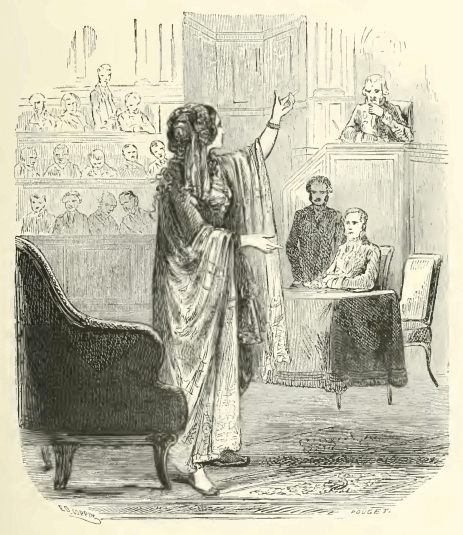
\includegraphics[width=\textwidth]{40202m.jpg}
\end{figure}

“The blush of mingled pride and modesty which suddenly suffused the
cheeks of the young woman, the brilliancy of her eye, and her highly
important communication, produced an indescribable effect on the
assembly. As for the count, he could not have been more overwhelmed if
a thunderbolt had fallen at his feet and opened an immense gulf before
him.

“‘Madame,’ replied the president, bowing with profound respect, ‘allow
me to ask one question; it shall be the last: Can you prove the
authenticity of what you have now stated?’

“‘I can, sir,’ said Haydée, drawing from under her veil a satin satchel
highly perfumed; ‘for here is the register of my birth, signed by my
father and his principal officers, and that of my baptism, my father
having consented to my being brought up in my mother’s faith,—this
latter has been sealed by the grand primate of Macedonia and Epirus;
and lastly (and perhaps the most important), the record of the sale of
my person and that of my mother to the Armenian merchant El-Kobbir, by
the French officer, who, in his infamous bargain with the Porte, had
reserved as his part of the booty the wife and daughter of his
benefactor, whom he sold for the sum of four hundred thousand francs.’
A greenish pallor spread over the count’s cheeks, and his eyes became
bloodshot at these terrible imputations, which were listened to by the
assembly with ominous silence.

“Haydée, still calm, but with a calmness more dreadful than the anger
of another would have been, handed to the president the record of her
sale, written in Arabic. It had been supposed some of the papers might
be in the Arabian, Romaic, or Turkish language, and the interpreter of
the House was in attendance. One of the noble peers, who was familiar
with the Arabic language, having studied it during the famous Egyptian
campaign, followed with his eye as the translator read aloud:

“‘I, El-Kobbir, a slave-merchant, and purveyor of the harem of his
highness, acknowledge having received for transmission to the sublime
emperor, from the French lord, the Count of Monte Cristo, an emerald
valued at eight hundred thousand francs; as the ransom of a young
Christian slave of eleven years of age, named Haydée, the acknowledged
daughter of the late lord Ali Tepelini, pasha of Yanina, and of
Vasiliki, his favorite; she having been sold to me seven years
previously, with her mother, who had died on arriving at
Constantinople, by a French colonel in the service of the Vizier Ali
Tepelini, named Fernand Mondego. The above-mentioned purchase was made
on his highness’s account, whose mandate I had, for the sum of four
hundred thousand francs.

“‘Given at Constantinople, by authority of his highness, in the year
1247 of the Hegira.

“‘Signed, El-Kobbir.’

“‘That this record should have all due authority, it shall bear the
imperial seal, which the vendor is bound to have affixed to it.’

“Near the merchant’s signature there was, indeed, the seal of the
sublime emperor. A dreadful silence followed the reading of this
document; the count could only stare, and his gaze, fixed as if
unconsciously on Haydée, seemed one of fire and blood. ‘Madame,’ said
the president, ‘may reference be made to the Count of Monte Cristo, who
is now, I believe, in Paris?’

“‘Sir,’ replied Haydée, ‘the Count of Monte Cristo, my foster-father,
has been in Normandy the last three days.’

“‘Who, then, has counselled you to take this step, one for which the
court is deeply indebted to you, and which is perfectly natural,
considering your birth and your misfortunes?’—‘Sir,’ replied Haydée, ‘I
have been led to take this step from a feeling of respect and grief.
Although a Christian, may God forgive me, I have always sought to
revenge my illustrious father. Since I set my foot in France, and knew
the traitor lived in Paris, I have watched carefully. I live retired in
the house of my noble protector, but I do it from choice. I love
retirement and silence, because I can live with my thoughts and
recollections of past days. But the Count of Monte Cristo surrounds me
with every paternal care, and I am ignorant of nothing which passes in
the world. I learn all in the silence of my apartments,—for instance, I
see all the newspapers, every periodical, as well as every new piece of
music; and by thus watching the course of the life of others, I learned
what had transpired this morning in the House of Peers, and what was to
take place this evening; then I wrote.’

\begin{figure}[ht]
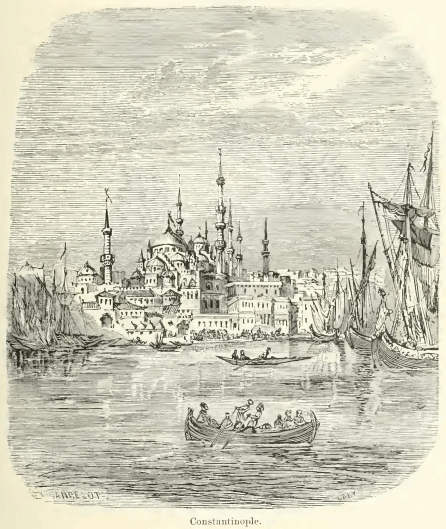
\includegraphics[width=\textwidth]{40204m.jpg}
\end{figure}

“‘Then,’ remarked the president, ‘the Count of Monte Cristo knows
nothing of your present proceedings?’—‘He is quite unaware of them, and
I have but one fear, which is that he should disapprove of what I have
done. But it is a glorious day for me,’ continued the young girl,
raising her ardent gaze to heaven, ‘that on which I find at last an
opportunity of avenging my father!’

“The count had not uttered one word the whole of this time. His
colleagues looked at him, and doubtless pitied his prospects, blighted
under the perfumed breath of a woman. His misery was depicted in
sinister lines on his countenance. ‘M. de Morcerf,’ said the president,
‘do you recognize this lady as the daughter of Ali Tepelini, pasha of
Yanina?’—‘No,’ said Morcerf, attempting to rise, ‘it is a base plot,
contrived by my enemies.’ Haydée, whose eyes had been fixed on the
door, as if expecting someone, turned hastily, and, seeing the count
standing, shrieked, ‘You do not know me?’ said she. ‘Well, I
fortunately recognize you! You are Fernand Mondego, the French officer
who led the troops of my noble father! It is you who surrendered the
castle of Yanina! It is you who, sent by him to Constantinople, to
treat with the emperor for the life or death of your benefactor,
brought back a false mandate granting full pardon! It is you who, with
that mandate, obtained the pasha’s ring, which gave you authority over
Selim, the fire-keeper! It is you who stabbed Selim. It is you who sold
us, my mother and me, to the merchant, El-Kobbir! Assassin, assassin,
assassin, you have still on your brow your master’s blood! Look,
gentlemen, all!’

“These words had been pronounced with such enthusiasm and evident
truth, that every eye was fixed on the count’s forehead, and he himself
passed his hand across it, as if he felt Ali’s blood still lingering
there. ‘You positively recognize M. de Morcerf as the officer, Fernand
Mondego?’—‘Indeed I do!’ cried Haydée. ‘Oh, my mother, it was you who
said, “You were free, you had a beloved father, you were destined to be
almost a queen. Look well at that man; it is he who raised your
father’s head on the point of a spear; it is he who sold us; it is he
who forsook us! Look well at his right hand, on which he has a large
wound; if you forgot his features, you would know him by that hand,
into which fell, one by one, the gold pieces of the merchant
El-Kobbir!” I know him! Ah, let him say now if he does not recognize
me!’ Each word fell like a dagger on Morcerf, and deprived him of a
portion of his energy; as she uttered the last, he hid his mutilated
hand hastily in his bosom, and fell back on his seat, overwhelmed by
wretchedness and despair. This scene completely changed the opinion of
the assembly respecting the accused count.

“‘Count of Morcerf,’ said the president, ‘do not allow yourself to be
cast down; answer. The justice of the court is supreme and impartial as
that of God; it will not suffer you to be trampled on by your enemies
without giving you an opportunity of defending yourself. Shall further
inquiries be made? Shall two members of the House be sent to Yanina?
Speak!’ Morcerf did not reply. Then all the members looked at each
other with terror. They knew the count’s energetic and violent temper;
it must be, indeed, a dreadful blow which would deprive him of courage
to defend himself. They expected that his stupefied silence would be
followed by a fiery outburst. ‘Well,’ asked the president, ‘what is
your decision?’

\begin{figure}[ht]
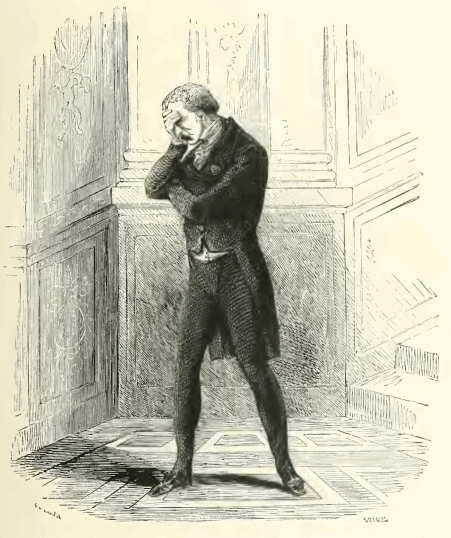
\includegraphics[width=\textwidth]{40206m.jpg}
\end{figure}

“‘I have no reply to make,’ said the count in a low tone.

“‘Has the daughter of Ali Tepelini spoken the truth?’ said the
president. ‘Is she, then, the terrible witness to whose charge you dare
not plead “Not guilty”? Have you really committed the crimes of which
you are accused?’ The count looked around him with an expression which
might have softened tigers, but which could not disarm his judges. Then
he raised his eyes towards the ceiling, but withdrew then, immediately,
as if he feared the roof would open and reveal to his distressed view
that second tribunal called heaven, and that other judge named God.
Then, with a hasty movement, he tore open his coat, which seemed to
stifle him, and flew from the room like a madman; his footstep was
heard one moment in the corridor, then the rattling of his
carriage-wheels as he was driven rapidly away. ‘Gentlemen,’ said the
president, when silence was restored, ‘is the Count of Morcerf
convicted of felony, treason, and conduct unbecoming a member of this
House?’—‘Yes,’ replied all the members of the committee of inquiry with
a unanimous voice.

“Haydée had remained until the close of the meeting. She heard the
count’s sentence pronounced without betraying an expression of joy or
pity; then drawing her veil over her face she bowed majestically to the
councillors, and left with that dignified step which Virgil attributes
to his goddesses.”
